\documentclass{article}
\PassOptionsToPackage{numbers,compress,sort}{natbib}
\usepackage[preprint]{neurips_2025}
\usepackage[utf8]{inputenc}
\usepackage[T1]{fontenc}
\usepackage{hyperref,url,booktabs,amsfonts,amsmath,amssymb,microtype}
\usepackage{xcolor,graphicx,array,pifont,makecell}
\usepackage[font=small,labelfont=bf,skip=3pt]{caption}
\usepackage[shortlabels]{enumitem}
\usepackage{listings}
\lstset{basicstyle=\ttfamily\scriptsize,columns=fullflexible,keepspaces=true,frame=tb,
  framesep=3pt,showstringspaces=false,upquote=true,aboveskip=6pt,belowskip=4pt}
\graphicspath{{../v12/figures/}{../../figures/}{../figures_own/}}
\hypersetup{pdftitle={How Should We Read ViT Attention Maps? A Fast-Weight Perspective},pdfauthor={Hongbo Huang},colorlinks=true,linkcolor=black,citecolor=blue!50!black,urlcolor=blue!50!black}
\newcommand{\up}{$^{\uparrow}$}
\newcommand{\dn}{$^{\downarrow}$}
\newcommand{\rsub}[1]{\refstepcounter{subsection}\paragraph{\thesubsection~~#1}}
\newcommand{\plabel}[3]{\makebox[#1][l]{\small\textbf{#2}~#3}}
\title{How Should We Read ViT Attention Maps?\\A Fast-Weight Perspective}
\author{Hongbo Huang\\Student ID: 50026755}
\begin{document}
\raggedbottom
\maketitle
\begin{abstract}
A patch can attract strong attention while returning a short value vector. We use the fast-weight view of attention to test how value lengths affect spatial maps and how those maps relate to classification. Norm weighting improves object localisation and human alignment in supervised DeiT. On Oxford-IIIT Pet, assigning each image's value lengths to positions ranked by another image reduces localisation. For classification, we directly remove individual patch contributions to the final classification token. Restricting the readout to this query improves agreement with changes in the class margin and reduces localisation on the same images. The spatial assignment of value lengths and the choice of receiving query thus explain different aspects of an attention map.

\end{abstract}

\section{Introduction}
A background patch can attract strong attention in a vision transformer~\citep{caron2021,darcet2024}. What evidence did the classifier use there? A deep token has already exchanged information with other positions. Even a strongly attended token can send a small vector to a query. Both observations complicate the familiar reading of a bright patch as important input.

\begin{figure}[!h]\centering
\begin{minipage}[c]{0.38\linewidth}
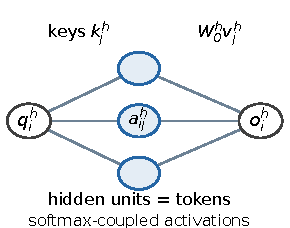
\includegraphics[width=\linewidth]{fast_weight_lens}
\end{minipage}\hfill
\begin{minipage}[c]{0.57\linewidth}\small
\textbf{Reading a bright patch}\\[3pt]
\textit{Image specificity.} How much of its score recurs across images?\\[3pt]
\textit{Spatial correspondence.} What links the token's grid position to its input evidence?\\[3pt]
\textit{Output contribution.} How large a value does the token send to the receiving query?
\end{minipage}
\caption{A head as a fast-weight network for one image. Keys and transformed values are its weights. The map places softmax activations at the source slots.}\label{fig:lens}
\end{figure}

How do these reading choices shape what a map explains? Using the fast-weight representation~\citep{wen2026mita} (Fig.~\ref{fig:lens}), we make three contributions.
\begin{enumerate}[nosep,leftmargin=1.65em,label=(\arabic*)]
\item We give an observable diagnostic for each assumption linking token activations to image evidence.
\item We test each change in readout against a matched control on three frozen checkpoints.
\item We show that position-based relocation hurts deep maps and that the choice of query can improve agreement with a classifier intervention while worsening localisation.
\end{enumerate}
\clearpage

\section{Related work}
\paragraph{From attention to a readable unit.} Vision transformers mix patch tokens by attention~\citep{dosovitskiy2021}. Fast-weight memory lets a network write temporary weights~\citep{schmidhuber1992}. Linear attention admits such an interpretation~\citep{schlag2021}, and softmax attention has connections to Hopfield memory~\citep{ramsauer2021}. We use MiTA's two-layer representation of softmax attention~\citep{wen2026mita} to identify choices made when displaying a frozen model's activations.

\paragraph{From a token to an image region.} Token identity can persist under contextual mixing~\citep{brunner2020,raghu2021}. Registers change the computation that produces high-norm tokens~\citep{darcet2024,jiang2025}, and no-op heads offer one account of outliers~\citep{bondarenko2023}. We instead vary how the same tokens are placed and weighted on a grid. Rollout, relevance propagation, gradient weighting and filtering offer other readings~\citep{abnar2020,chefer2021,chefer2021generic,ayyar2025}. Prior norm analyses incorporate transformed values~\citep{kobayashi2020,zhu2024}. GlobEnc, ALTI and TokenTM also track transformations across layers~\citep{modarressi2022,ferrando2022,wu2024tokentm}. Our local comparisons isolate the spatial assignment of value lengths and the choice of receiving query.

\paragraph{Which output is explained?} The explanatory value of attention depends on the test~\citep{jain2019,wiegreffe2019}. CAM targets a specified class~\citep{zhou2016}. Value zeroing measures contextual mixing~\citep{mohebbi2023}. Parameter sensitivity, supervision, occlusion and spatial priors can all affect map evaluation~\citep{adebayo2018,walmer2023,bluecher2024,kuang2026}. We compare spatial alignment with a direct intervention on the final classification-token (CLS) pathway.

\section{A fast-weight framework for reading attention}
\label{sec:method}
For query $i$, source $j$ and head $h$, let $z_j^h=W_O^h v_j^h$ be the transformed value. With affine query, key and value projections, the attention output before residual addition is
\begin{equation}
 o_i=b_O+\sum_{h,j}a^h_{ij}z^h_j,\qquad
 a^h_{ij}=\mathrm{softmax}_j(q_i^{h\top}k_j^h/\sqrt{d}).
\label{eq:attn}
\end{equation}
For a fixed image, $k_j^h/\sqrt d$ and $z_j^h$ act as the input and output weights of a two-layer network in $q_i^h$. Received attention (R0) assigns $s_j=\sum_{h,i}a^h_{ij}$ to patch slot $j$. It sums over all queries, including CLS, and reports the 196 patch scores. We test three assumptions behind that last step using diagnostic proxies~\citep{bau2017} and paired changes to the readout.

\paragraph{Image specificity (C1).} A bright slot may reflect a recurring spatial pattern. We estimate how much spatial variance a held-out mean map explains and subtract that map from each image's scores. Subtracting a centred Gaussian scaled to the mean map's spatial standard deviation controls for a radial prior.

\paragraph{Spatial correspondence (C2).} A patch slot contains contextual information. We train a linear probe to decode each token's grid index and redistribute $s_j$ by its predicted position probabilities. A blur matched in mean squared displacement tests whether redistribution adds anything beyond smoothing. Index accuracy measures recoverable position information. The input origin of a token's content remains unknown.

\paragraph{Output contribution (C3).} Activation omits the length and direction of the vector sent to a query. We measure the share of attention on patches with block-input norm above three times the image median. C3 weights each activation by its transformed-value length, $c_j=\sum_{h,i}a_{ij}^h\|z_j^h\|_2$. Its control simply zeros received attention on the high-norm patches. C3 uses no threshold. For a single query--source pair,
\[
 \Big\|\sum_h a^h_{ij} z_j^h\Big\|_2 \leq \sum_h a^h_{ij}\|z_j^h\|_2.
\]
The left side retains cancellation between heads. C3 sums the right side over queries. Both measures are local to the attention branch. Neither includes residuals, MLPs or subsequent token mixing.
\clearpage

\section{Testing the three assumptions on frozen models}
\label{sec:exp}
\begin{figure}[!h]\centering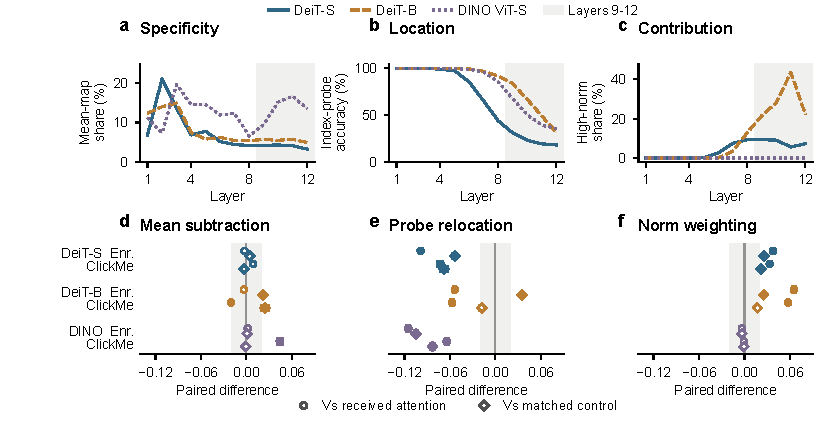
\includegraphics{diagnosis_correction_bridge}
\caption{Each column pairs a diagnostic (a--c) with a change in readout (d--f). Top curves give per-layer means and 95\% intervals on ImageNet-S (a,c) or 2,000 held-out images (b). Shading marks layers 9--12. Bottom points compare the modified reading with R0 (circle) and its matched control (diamond) on the two alignment metrics. Bars are unadjusted paired 95\% image-bootstrap intervals. Filled points clear both zero (interval) and $\pm0.02$ (mean). The link between diagnostic and benefit is assessed post hoc.}\label{fig:diag}
\end{figure}

\paragraph{Design and decision rule.} We evaluated frozen DeiT-S/B~\citep{touvron2021} and DINO ViT-S/16~\citep{caron2021}, summing maps across layers 9--12 unless specified. On ImageNet-S~\citep{gao2023} (12,419 images), enrichment compares the foreground rate among top-ranked patches with the rate at the same radii. On ClickMe~\citep{linsley2019,fel2022} (17,408 images), alignment is the own-image minus other-image correlation with human maps (Spearman). Deletion integrates least- minus most-important-first top-1 retention on 2,000 images. Another 4,000 ImageNet images~\citep{deng2009} were split equally for probe training and calibration. A higher or lower verdict requires a paired 95\% bootstrap interval excluding zero and an absolute mean difference of at least 0.02 (0.05 for deletion). All other differences are termed comparable, a decision category that includes imprecise estimates.

\paragraph{What changes under matched controls?} In deep layers the held-out mean pattern was mostly radial, position decoding weakened with depth, and late high-norm attention was concentrated in the supervised models (Fig.~\ref{fig:diag}a--c). Mean subtraction's sole gain over R0, on DINO ClickMe, was comparable to Gaussian subtraction. In DeiT-B it beat the Gaussian on all three metrics but yielded no gain over R0. Deep probe relocation lowered all nine model--metric scores relative to R0 and underperformed matched blur in DeiT-S and DINO. In supervised DeiT-S/B, value weighting improved enrichment by 0.038/0.065 and ClickMe alignment by 0.033/0.058 over R0. Three of the four gains also cleared the high-norm control. The fourth, DeiT-B ClickMe, was 0.017 above control. Top-1 deletion gains of 0.017/0.029 fell below the registered 0.05 margin.

\paragraph{Registered predictions.} R1 held in all nine tests: deep C3 in DINO was comparable to R0 on all three metrics, as was early C2 (layers 1--4) on both alignment metrics in all three models. R2 predicted four supervised alignment gains from combining C3, C2 and C1. One score was higher, one comparable and two lower (\emph{partly holds}). R3 held: neither a test-time register nor the released MiTA model exceeded DeiT-S on either alignment metric under the decision rule. MiTA also differs in training and preprocessing. The primary contrasts were combined changes versus R0 and each change versus its matched control. Other individual contrasts with R0 were descriptive except for R1. The protocol followed pilot observations (App.~\ref{app:setup}).
\clearpage
\section{What the spatial weights encode}
We ran an exploratory transfer test on Oxford-IIIT Pet~\citep{parkhi2012pets} with the same frozen DeiT-S. We selected 384 test images by a fixed hash of their filenames. For 383 crops, both foreground and background patches were available. To test whether the image's own assignment matters, we paired images and placed each recipient's sorted value lengths at positions ranked by its donor, independently for each layer and head. A second control shuffled lengths within rings of equal distance to the image centre. Both keep the lengths available to each head. A norm-only reading keeps each head's total attention to patches and spreads it uniformly before weighting by length.

\begin{center}\begin{minipage}{\linewidth}
\captionof{table}{Spatial readouts on Oxford-IIIT Pet (DeiT-S, layers 9--12). All rows score the same 383 masks. The paired differences and image-bootstrap intervals refer to same-ring enrichment. AUROC compares the scores of foreground and background patches.}
\label{tab:pets}\centering\small\setlength{\tabcolsep}{5pt}
\begin{tabular}{@{}lrrr@{}}
\toprule
Reading & Enrichment & Difference from C3 [95\% CI] & AUROC \\
\midrule
Received attention (R0) & 0.141 & $-$0.019 [$-$0.023, $-$0.015] & 0.788 \\
Projected value norm (C3) & 0.160 & --- & 0.817 \\
Unprojected value norm & 0.163 & 0.004 [0.003, 0.005] & 0.822 \\
Norm after summing heads & 0.156 & $-$0.003 [$-$0.005, $-$0.002] & 0.809 \\
Value norm only & 0.120 & $-$0.040 [$-$0.048, $-$0.032] & 0.757 \\
Donor-image positions & 0.137 & $-$0.022 [$-$0.026, $-$0.019] & 0.787 \\
Within-ring permutation & 0.138 & $-$0.021 [$-$0.025, $-$0.018] & 0.793 \\
\bottomrule
\end{tabular}

\end{minipage}\end{center}

Reassigning lengths across images or within rings lowers enrichment by 0.022 and 0.021 relative to C3 (Table~\ref{tab:pets}). The donor-pair bootstrap gives an interval of [0.019, 0.026] for the former difference. Norm-only scoring also loses 0.040. Thus both the spatial variation in attention and the assignment of lengths within the image contribute to the observed alignment. Using the unprojected lengths gives a slightly higher score. Summing vectors across heads before taking their norm lowers enrichment by 0.003. Both alternative length measures preserve most of the improvement over R0.

\paragraph{Which receiving query matters?} On 128 of the pet images we removed one source patch's value term at a time from the last CLS attention output, holding attention fixed. We recomputed the remaining block and classifier, then ranked all 196 patches by the absolute change in the original top-two logit margin. Restricting C3 to the CLS query improved its within-image rank correlation with this intervention by 0.041 [0.026, 0.057]. After seeing that result, we scored the same layer-12 rankings against the masks. The same query restriction reduced both enrichment and AUROC (Table~\ref{tab:cls}). The paired 95\% interval for the AUROC change was $[-0.110,-0.074]$.

\begin{center}\begin{minipage}{\linewidth}
\captionof{table}{Classifier sensitivity and foreground alignment for layer-12 readouts on the same 128 images. Entries are image means. Margin Spearman compares the readout with the measured patch effects on the CLS pathway. Net magnitude takes the norm after summing head vectors, allowing them to cancel.}
\label{tab:cls}\centering\small\begin{tabular}{@{}lrrr@{}}
\toprule
Layer-12 readout & Margin Spearman & Enrichment & AUROC \\
\midrule
All queries, attention & 0.696 & 0.117 & 0.754 \\
All queries, sum of magnitudes & 0.705 & 0.127 & 0.769 \\
CLS, attention & 0.730 & 0.081 & 0.666 \\
CLS, sum of magnitudes & 0.747 & 0.095 & 0.678 \\
CLS, net magnitude & 0.756 & 0.098 & 0.678 \\
\bottomrule
\end{tabular}

\end{minipage}\end{center}

\section{Discussion and conclusion}
Keeping the image-specific patch positions of value lengths within each head improves the spatial readout. The observed advantage depends on the checkpoint, object geometry and the endpoint used to measure model behaviour. The pet experiment covers one supervised checkpoint and a narrow image domain. Within the original study, supervision, classifier head and preprocessing differ across checkpoints. The input deletion experiment changes the context at every later layer, and ClickMe images may overlap model training data. Public image and human-map datasets also reflect the choices of their photographers and annotators. These limits favour reporting localisation and behavioural sensitivity together when interpreting an attention map.

\label{main:end}
\clearpage
{\small\bibliographystyle{plainnat}\bibliography{references}}
\clearpage\appendix
% =====================================================================================================
% Appendix: experimental details (A), additional results (B), analysis of probe relocation (C),
% example maps (D), exploratory tests (E) and key code (F).
% =====================================================================================================

\counterwithin{figure}{section}
\counterwithin{table}{section}
\captionsetup{skip=5pt}
\raggedbottom

\section{Experimental details}
\label{app:setup}

\paragraph{Models.} All models are frozen ViTs with $16{\times}16$ patches on $224{\times}224$ inputs, taken from timm~\citep{wightman2019}. \emph{DeiT-S and DeiT-B}~\citep{touvron2021}: \texttt{deit\_small\_patch16\_224.fb\_in1k} and \texttt{deit\_base\_patch16\_224.fb\_in1k} (resize to 248, centre crop 224: a crop ratio of 0.9). \emph{DINO ViT-S/16}~\citep{caron2021}: \texttt{vit\_small\_patch16\_224.dino} with the official DINO linear head (resize to 256, centre crop 224: a crop ratio of 0.875). \emph{DeiT-S with a test-time register}~\citep{jiang2025}: the activations of eight feed-forward units in layers 4 and 5 are moved to one added register token, which is left out of every map, like CLS. The units were selected on 500 ImageNet-S images, where they reduce the number of high-norm patch tokens (counted per layer) by 92.75\% and keep 99.0\% of the predictions; on the other 11,919 images the reduction is 91.5\%, and ImageNet accuracy stays at 79.8\%. For DeiT-B the same search found no such units (44.9\% reduction with 32 units), so we report the register for DeiT-S only. \emph{Top-$k$ training}: the DeiT-S checkpoint released with MiTA~\citep{wen2026mita} (25 summary slots, $k=25$), with its own preprocessing (crop ratio 0.875). It differs from our DeiT-S in training and preprocessing, so its row in Table~\ref{tab:main} is not a controlled comparison; its deletion score is undefined because its summary slots pool fixed regions of the full grid. Both model-side fixes are tested at size S only; in a preliminary comparison with an earlier protocol, top-$k$ training scored 0.011 lower in object enrichment than its baseline at size S but 0.037 higher at size Tiny, so the result should not be read beyond DeiT-S.

\paragraph{Attention conventions.} With $x$ the block input after its first layer norm, projections include the checkpoint's biases:
\[
q_i^h=W_Q^hx_i+b_Q^h,\quad k_j^h=W_K^hx_j+b_K^h,\quad v_j^h=W_V^hx_j+b_V^h.
\]
Equation~\ref{eq:attn} includes the output bias $b_O$ and describes the attention branch before residual addition, with dropout inactive at evaluation. $W_O^h$ is the head's slice of the output projection. C3 assigns the per-head vector magnitudes to patches; the shared output bias is not assigned to any patch. The fixed-image two-layer representation uses the coupled softmax activation, rather than an elementwise nonlinearity.

\paragraph{Data.} \emph{Execution test}: 5,000 randomly drawn ImageNet validation images~\citep{deng2009}. \emph{ImageNet-S}~\citep{gao2023}: all 12,419 validation images with segmentation masks; stored enrichment is finite for 12,150 (12,144 for DINO). Historical records include all-foreground grids scored zero. Appendix~\ref{app:explore} gives the cohort sensitivity check. Deletion uses a fixed random subset of 2,000. \emph{ClickMe}~\citep{linsley2019,fel2022}: the 17,408-image validation split released with Harmonization (17 \texttt{val-*.tfrecords} shards). This split name does not identify the original ImageNet split of each image. Images are resized from $256{\times}256$ to $224{\times}224$ without cropping; heatmaps are resized to $64{\times}64$, blurred with a $10{\times}10$ Gaussian ($\sigma=10$), then resized to $224{\times}224$ (bilinear interpolation). \emph{Held-out set}: 4,000 ImageNet validation images excluded from map-quality and execution evaluation; 2,000 train probes and 2,000 provide mean maps, probe-test accuracies and blur calibration. Our near-duplicate check matched 2 of 4,002 candidate ImageNet validation images to ClickMe records; this does not establish every ClickMe image's training-set membership. Possible overlap with model training images limits generalisation claims.

\paragraph{Diagnostics.} All three are computed per layer. \emph{Specificity}: with $\bar s$ the mean received-attention map of the held-out images and $\operatorname{Var}_j$ the variance over the 196 patches of one image, the share explained is $1-\sum_x\operatorname{Var}_j(s-\bar s)\,/\sum_x\operatorname{Var}_j(s)$, summed over the ImageNet-S images $x$. \emph{Location}: the top-1 accuracy of the linear position probe on the 196 patch tokens of each of 2,000 held-out images. \emph{Contribution}: the share of received attention on high-norm tokens, on the ImageNet-S images. The high-norm threshold (three times the median, defined below) is an operational definition fixed before the experiments; we did not test other thresholds. The correction itself uses no threshold.

\paragraph{Corrections and matched controls.} Scores are computed per layer and summed over layers 9--12 without per-layer rescaling, except for the C1 control's calibration described below. Queries include all 197 tokens; maps contain 196 patches. Negative C1 scores are retained for ranking, without clipping.
\emph{Mean-map subtraction} computes $\sum_\ell(s_\ell-\bar s_\ell)$ using the 2,000 calibration images. With $S=\sum_\ell s_\ell$ and $\bar S=\sum_\ell\bar s_\ell$, its control is $S-G\,\operatorname{sd}_j(\bar S)/\operatorname{sd}_j(G)$, where $G$ is a centred isotropic Gaussian ($\sigma=3.5$ patches). Calibration thus uses the \emph{summed} mean map.
\emph{Probe relocation} computes $r_p=\sum_j s_jP_\ell(p\mid x_j)$, preserving total score. One linear 196-way classifier per model/layer is trained on standardised tokens after the first layer norm: cross-entropy, Adam, learning rate 0.01, 30 epochs, token minibatches of 4,096, seed 0. Feature means/standard deviations use only the 2,000 training images; standard deviations are floored at $10^{-6}$. Its Gaussian control is a row-normalised kernel $K_{jp}\propto\exp(-\lVert p-j\rVert^2/(2\sigma_\ell^2))$. The width (0.7--2.9 patches) matches
\[
D_\ell=\frac{1}{2000N}\sum_{x,j,p}P_\ell(p\mid x_j)\lVert p-j\rVert^2
\]
on calibration images, using uniform averaging over source patch indices. Matching uses uniform source indices. ClickMe uses the same crop-trained probe and blur on resized full images, introducing a potential geometry mismatch.
\emph{Contribution weighting} computes $c_j=\sum_{h,i}a_{ij}^h\lVert W_O^hv_j^h\rVert_2$, a sum of per-head norm-weighted terms related to \citet{kobayashi2020}. Summing magnitudes before aggregating across heads omits cross-head cancellation; residual addition, subsequent normalisation and later-layer computation are outside this score. The control zeros received attention at high-norm patches: block-input norm greater than three times the image's median patch norm, using the midpoint median. C3 itself has no high-norm threshold.
\emph{All three corrections}: contribution weighting, probe relocation, then subtraction of the held-out mean of the resulting map, per layer before summation.

\paragraph{Metrics.} \emph{Same-ring object enrichment.} A patch is valid if it contains at least one non-ignored pixel, and is an object patch if at least half of its non-ignored pixels belong to the image's class mask. We select as many top-scoring patches as there are object patches. For every ring of patches at the same distance from the grid centre, we take the object rate among its selected patches minus that among all its patches, and average over rings, weighted by their selected patches. Invalid patches are excluded from selection and ring baselines. Ties are broken with the fixed seeded perturbation used in the original runs. A purely radial map scores zero in expectation over tie-breaking.
\emph{Image-specific ClickMe alignment.} The map is upsampled to $224{\times}224$ and correlated (Spearman, over pixels) with the image's own human map; we subtract its correlation with the previous image's human map within each batch (\texttt{roll(1)}; batch size 64). For an image-independent map, these differences average to zero over the paired set because the control permutes the same human maps; individual-image differences need not be zero. This removes fixed-prior alignment on average, without guaranteeing invariance to a prior mixed into an image-dependent map.
\emph{Deletion score.} Patches are ranked once by the original map. At removal budgets $0,1,2,4,8,16,32,64,98,147$, we record the binary indicator that the original top-1 prediction is preserved. Tokens are dropped after positional embedding; CLS and any register remain. We use an SRG-style LIF--MIF area difference~\citep{bluecher2024}, adapting the value function from class probability to top-1 preservation. Areas use trapezoidal integration over removed-patch fraction $b/196$, from 0 to $147/196$.
\emph{Validity of the metrics.} A random map, a centred Gaussian and the mean map all score within 0.004 of zero on enrichment and on ClickMe alignment (the two image-independent maps have exactly zero mean on the latter, up to numerical precision); on deletion the centred Gaussian scores 0.110, 0.099 and 0.140 (DeiT-S, DeiT-B, DINO ViT-S), which is why every correction is compared with a matched control.
\emph{Statistics.} One value per image; paired image-bootstrap with 1,000 resamples, seed 0 and 95\% percentile intervals. A difference is \emph{higher} (\textit{h}) or \emph{lower} (\textit{l}) if its interval excludes zero and its absolute mean reaches 0.02 (0.05 for deletion), and \emph{comparable} (\textit{c}) otherwise. The comparable category also covers imprecise differences. Intervals are unadjusted for multiple comparisons. Resampling holds checkpoints, probes and the within-batch ClickMe pairing fixed, excluding uncertainty from training, probe fitting or alternative pairings. Because the control reuses human maps within each batch, ClickMe score rows are not independent pairings.

\paragraph{GAE reference.} The gradient-based reference~\citep{chefer2021generic} targets the unmodified model's predicted top-1 logit and uses all 12 attention layers. Starting with $R=I$, each layer updates $R\leftarrow R+\operatorname{mean}_h[(\nabla_{A^h}f_c\odot A^h)_+]R$, then takes the final CLS-to-patch row. It is class-specific and spans all layers, whereas R0/C1--C3 are class-agnostic and sum layers 9--12. Its scores provide descriptive context rather than a matched single-component ablation.

\paragraph{Registered predictions.} The protocol was frozen before formal runs, after smoke tests on 32--64 images and earlier exploratory observations documented in \texttt{docs/preregistration.md}. Historical P4/P3/P6 map to R1/R2/R3; definitions, margins and verdicts are unchanged. R2 has three possible outcomes: holds (4/4 higher), partly holds (1--3) and does not hold (0). Primary contrasts were the combination versus R0 and each correction versus its matched control, without a registered direction for the latter. Other correction--R0 contrasts are descriptive, except R1's registered negative controls. Prior execution/diagnostic results had been seen, making the last two rows of Table~\ref{tab:app-registered} replications. Diagnosis--benefit interpretation and supplementary mechanism analyses are post hoc.

\begin{table}[!htbp]
\caption{Registered predictions and outcomes (centre-controlled metrics: enrichment and ClickMe alignment).}
\label{tab:app-registered}
\centering\footnotesize
\setlength{\tabcolsep}{4pt}
\begin{tabular}{@{}l>{\raggedright\arraybackslash}p{3.55in}>{\raggedright\arraybackslash}p{1.35in}@{}}
\toprule
 & Prediction & Outcome\\
\midrule
R1 & Contribution weighting is comparable to received attention in DINO ViT-S on all three metrics & holds (3 of 3 cells)\\
R1 & Relocation at layers 1--4 is comparable to received attention on the centre-controlled metrics in all models & holds (6 of 6 cells)\\
R2 & All three corrections together are higher than received attention on the centre-controlled metrics in DeiT-S and DeiT-B & partly holds (1 higher: DeiT-B ClickMe; 1 comparable; 2 lower)\\
R3 & Neither model-side change is higher than DeiT-S received attention on the centre-controlled metrics & holds (4 of 4 cells)\\
\midrule
-- & Execution agreement rises with $k$ and exceeds that of random sets at every $k$ & holds in all models\\
-- & Probe accuracy falls with depth; the share of attention on high-norm tokens peaks in layers 6--12 of the supervised models and is below 1\% in every layer of DINO ViT-S & holds in all models\\
\bottomrule
\end{tabular}
\end{table}

\paragraph{Compute and code.} The original experiments took about 19 NVIDIA L4 GPU hours. Code, configurations, fixed splits, checkpoint revisions and recorded provenance: \url{https://github.com/hhuang999/vit-fastweight-lens}. The release supplies \texttt{configs/}, \texttt{data/splits/} and \texttt{docs/provenance/}; unavailable historical environment fields remain unknown. The exploratory protocols, scripts and results accompanying this study are in the supplied source under \texttt{research/v13/}.

% =====================================================================================================
\section{Additional results}
\label{app:more}

These results support the framework at different levels: execution and parameter sensitivity check internal dependence, while paired comparisons and supplementary analyses assess map quality and proposed interpretations.
\suppressfloats[t]

\begin{center}\begin{minipage}{\linewidth}
\captionof{table}{Complete scores for the original tests, layers 9--12 unless indicated. Arrows mark higher/lower scores versus received attention (DeiT-S for model-side rows). Diamonds indicate higher scores than the matched control. Bold indicates higher than both. Untagged tested cells are comparable. GAE uses gradients and all 12 layers. Dashes indicate unavailable comparisons.}
\label{tab:main}
\centering\footnotesize\setlength{\tabcolsep}{2.6pt}
% v9 presentation; all values and verdicts are read unchanged from results/.
\begin{tabular}{@{}l@{\hspace{4pt}}rrr@{\hspace{7pt}}rrr@{\hspace{7pt}}rrr@{}}
\toprule
 & \multicolumn{3}{c}{DeiT-S} & \multicolumn{3}{c}{DeiT-B} & \multicolumn{3}{c}{DINO ViT-S}\\
\cmidrule(r{6pt}){2-4}\cmidrule(r{6pt}){5-7}\cmidrule{8-10}
Reading & Enr. & Click. & Del. & Enr. & Click. & Del. & Enr. & Click. & Del.\\
\midrule
Received attention & 0.140 & 0.157 & 0.236 & 0.080 & 0.107 & 0.169 & 0.199 & 0.208 & 0.285 \\
Contribution weighting & \textbf{0.178}$^{\uparrow\diamond}$ & \textbf{0.190}$^{\uparrow\diamond}$ & 0.253 & \textbf{0.146}$^{\uparrow\diamond}$ & 0.165$^{\uparrow}$ & 0.198 & 0.196 & 0.207 & 0.285 \\
\quad zero high-norm tokens & 0.152 & 0.168 & 0.241 & 0.121$^{\uparrow}$ & 0.148$^{\uparrow}$ & 0.186 & 0.199 & 0.208 & 0.285 \\
Mean-map subtraction & 0.138 & 0.165 & 0.208 & 0.077$^{\diamond}$ & 0.087$^{\downarrow\diamond}$ & 0.144$^{\diamond}$ & 0.201 & 0.252$^{\uparrow}$ & 0.233$^{\downarrow}$ \\
\quad subtract centre Gaussian & 0.133 & 0.168 & 0.167$^{\downarrow}$ & 0.056$^{\downarrow}$ & 0.062$^{\downarrow}$ & 0.024$^{\downarrow}$ & 0.200 & 0.253$^{\uparrow}$ & 0.232$^{\downarrow}$ \\
Probe relocation & 0.041$^{\downarrow}$ & 0.084$^{\downarrow}$ & 0.076$^{\downarrow}$ & 0.027$^{\downarrow\diamond}$ & 0.050$^{\downarrow}$ & 0.051$^{\downarrow}$ & 0.084$^{\downarrow}$ & 0.143$^{\downarrow}$ & 0.141$^{\downarrow}$ \\
\quad matched blur & 0.095$^{\downarrow}$ & 0.152 & 0.181$^{\downarrow}$ & $-$0.008$^{\downarrow}$ & 0.068$^{\downarrow}$ & 0.097$^{\downarrow}$ & 0.189 & 0.226 & 0.287 \\
All three corrections & 0.059$^{\downarrow}$ & 0.123$^{\downarrow}$ & 0.076$^{\downarrow}$ & 0.079 & 0.137$^{\uparrow}$ & 0.085$^{\downarrow}$ & 0.088$^{\downarrow}$ & 0.177$^{\downarrow}$ & 0.090$^{\downarrow}$ \\
\midrule
+ test-time register & 0.152 & 0.169 & 0.236 & -- & -- & -- & -- & -- & -- \\
Top-$k$ training (MiTA) & 0.100\dn & 0.115\dn & -- & -- & -- & -- & -- & -- & -- \\
GAE (reference) & 0.204 & 0.234 & 0.345 & 0.196 & 0.213 & 0.308 & 0.221 & 0.234 & 0.418 \\
\bottomrule
\end{tabular}

\end{minipage}\end{center}
\begin{samepage}\paragraph{Execution test.} The $14{\times}14$ grid is pooled into 16 overlapping regions. In every layer/head, each region's mean query selects its top-$k$ keys; CLS retains its own set. Sets from an unmodified forward pass restrict every query to its region's set in all 12 layers simultaneously. Top-$k$ sets beat equal-size random sets at every tested $k$ (4--128) in all models, and agreement rises with $k$ (Fig.~\ref{fig:app-ksweep}). The dotted attention-removed baseline alone uses uniform crop ratio 0.875; solid/dashed DeiT curves use 0.9.

\par\end{samepage}
\begin{center}\begin{minipage}{3.6in}
\centering
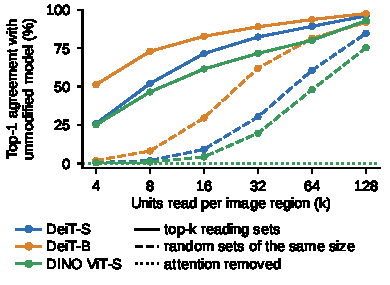
\includegraphics[width=3.25in]{execution_k_sweep}
\captionof{figure}{Top-1 agreement on 5,000 ImageNet images with region-selected top-$k$ units (solid), random units (dashed) or attention removed (dotted). Stored 95\% intervals are at most $\pm1.5$ percentage points. Dotted curves use crop ratio 0.875 for all models; other curves use each checkpoint's main preprocessing.}
\label{fig:app-ksweep}
\end{minipage}\end{center}

\paragraph{Diagnostics per layer.} Table~\ref{tab:app-diag} lists the diagnostics plotted in Fig.~\ref{fig:diag}a--c and the uncorrected per-layer ClickMe alignment. Two further details complement the table. First, in layers 9--12, 82--98\% of the variance of the mean map is explained by the distance from the grid centre. Second, averaged over layers 9--12, the mean value-vector norm $\lVert v_j\rVert$ of high-norm tokens is 0.29 (DeiT-S) and 0.23 (DeiT-B) times the median of the other patches (measured on 11,919 ImageNet-S images using uniform crop ratio 0.875, unlike the main DeiT evaluation at 0.9).

\paragraph{Recovery at the last layer.} In the supervised models, single-layer received attention is worse at layer 12 than at the best of layers 8--11 (ClickMe values in Table~\ref{tab:app-diag}). Applied to layer 12, contribution weighting recovers 62\% and 33\% of this drop on enrichment (DeiT-S, DeiT-B), 31\% and 45\% on ClickMe alignment, and 8\% and 29\% on deletion. The other two corrections make layer 12 worse.

\begin{table}[!htbp]
\caption{Per-layer diagnostics (Fig.~\ref{fig:diag}a--c) and uncorrected ClickMe alignment (last three columns). S, B, D: DeiT-S, DeiT-B, DINO ViT-S; probe chance: 0.5\%. Values are rounded; DINO layers 9--12 have exactly zero high-norm attention on this dataset.}
\label{tab:app-diag}
\centering
% Per-layer diagnostics, generated from results/diagnose.csv by diag_table.py.
\footnotesize
\setlength{\tabcolsep}{2.6pt}
\begin{tabular}{r >{\centering\arraybackslash}p{0.8cm} >{\centering\arraybackslash}p{0.8cm} >{\centering\arraybackslash}p{0.8cm} >{\centering\arraybackslash}p{0.8cm} >{\centering\arraybackslash}p{0.8cm} >{\centering\arraybackslash}p{0.8cm} >{\centering\arraybackslash}p{0.8cm} >{\centering\arraybackslash}p{0.8cm} >{\centering\arraybackslash}p{0.8cm} >{\centering\arraybackslash}p{1.05cm} >{\centering\arraybackslash}p{1.05cm} >{\centering\arraybackslash}p{1.05cm}}
\toprule
 & \multicolumn{3}{c}{\makecell{Specificity:\\mean-map share (\%)}} & \multicolumn{3}{c}{\makecell{Location:\\probe accuracy (\%)}} & \multicolumn{3}{c}{\makecell{Contribution:\\high-norm share (\%)}} & \multicolumn{3}{c}{\makecell{Map quality:\\ClickMe alignment}} \\
\cmidrule(lr){2-4}\cmidrule(lr){5-7}\cmidrule(lr){8-10}\cmidrule(lr){11-13}
Layer & S & B & D & S & B & D & S & B & D & S & B & D \\
\midrule
1 & 6.8 & 12.4 & 11.2 & 100.0 & 100.0 & 99.9 & 0.0 & 0.0 & 0.0 & $-$0.108 & $-$0.111 & $-$0.089 \\
2 & 21.2 & 14.0 & 7.4 & 100.0 & 100.0 & 100.0 & 0.0 & 0.0 & 0.0 & 0.007 & 0.041 & 0.064 \\
3 & 13.7 & 15.0 & 19.7 & 99.9 & 100.0 & 99.9 & 0.0 & 0.0 & 0.0 & 0.081 & 0.004 & 0.056 \\
4 & 6.9 & 7.5 & 14.6 & 99.0 & 100.0 & 99.8 & 0.0 & 0.0 & 0.0 & 0.132 & 0.110 & 0.140 \\
5 & 7.8 & 5.8 & 14.6 & 97.5 & 99.9 & 99.6 & 0.1 & 0.0 & 0.0 & 0.148 & 0.130 & 0.150 \\
6 & 5.2 & 6.2 & 11.9 & 85.3 & 99.5 & 98.9 & 2.6 & 0.0 & 0.0 & 0.136 & 0.151 & 0.167 \\
7 & 4.4 & 5.4 & 12.4 & 65.0 & 96.8 & 95.9 & 7.4 & 3.5 & 0.0 & 0.147 & 0.131 & 0.150 \\
8 & 4.2 & 5.4 & 6.6 & 43.9 & 91.8 & 85.6 & 9.3 & 12.9 & 0.0 & 0.149 & 0.118 & 0.170 \\
9 & 4.2 & 5.7 & 9.5 & 31.0 & 83.6 & 67.4 & 9.3 & 21.5 & 0.0 & 0.184 & 0.112 & 0.198 \\
10 & 4.3 & 5.5 & 15.2 & 23.1 & 66.8 & 50.5 & 9.1 & 28.1 & 0.0 & 0.171 & 0.139 & 0.207 \\
11 & 4.1 & 5.8 & 16.7 & 19.4 & 49.2 & 39.2 & 5.6 & 43.5 & 0.0 & 0.149 & 0.120 & 0.211 \\
12 & 3.3 & 5.0 & 13.6 & 18.1 & 31.8 & 35.7 & 7.2 & 22.2 & 0.0 & 0.098 & 0.023 & 0.179 \\
\bottomrule
\end{tabular}

\end{table}

\begin{table}[!tbp]
\caption{Paired differences, layers 9--12: mean, 95\% image-bootstrap interval and verdict (\textit{h}/\textit{c}/\textit{l}: higher/comparable/lower). Margins: 0.02 (enrichment/ClickMe), 0.05 (deletion); intervals unadjusted. Samples: App.~\ref{app:setup}. Top: descriptive correction--R0 contrasts and the primary combination--R0 contrasts. Bottom: primary correction--control contrasts. Registered negative controls are also discussed in App.~\ref{app:setup}.}
\label{tab:app-paired}
\centering
% Paired differences: blocks copied verbatim from repo/paper/tables/appendix/paired_differences.tex by
% make/make_paired_table.py (titles simplified, numbers unchanged).
\footnotesize
\setlength{\tabcolsep}{4pt}
\renewcommand{\arraystretch}{1.08}
\begin{tabular}{lccc}
\toprule
Model & Same-ring enrichment & ClickMe alignment & Deletion score \\
\midrule
\multicolumn{4}{l}{\textit{Contribution weighting $-$ received attention}} \\
DeiT-S & 0.038 {\fontsize{8}{9}\selectfont [0.036, 0.039]}\,\textit{h} & 0.033 {\fontsize{8}{9}\selectfont [0.032, 0.034]}\,\textit{h} & 0.017 {\fontsize{8}{9}\selectfont [0.013, 0.021]}\,\textit{c} \\
DeiT-B & 0.065 {\fontsize{8}{9}\selectfont [0.063, 0.067]}\,\textit{h} & 0.058 {\fontsize{8}{9}\selectfont [0.056, 0.059]}\,\textit{h} & 0.029 {\fontsize{8}{9}\selectfont [0.024, 0.034]}\,\textit{c} \\
DINO ViT-S & $-$0.004 {\fontsize{8}{9}\selectfont [$-$0.004, $-$0.003]}\,\textit{c} & $-$0.001 {\fontsize{8}{9}\selectfont [$-$0.001, $-$0.001]}\,\textit{c} & 0.000 {\fontsize{8}{9}\selectfont [$-$0.003, 0.004]}\,\textit{c} \\
\addlinespace[2pt]
\multicolumn{4}{l}{\textit{Mean-map subtraction $-$ received attention}} \\
DeiT-S & $-$0.002 {\fontsize{8}{9}\selectfont [$-$0.003, $-$0.002]}\,\textit{c} & 0.009 {\fontsize{8}{9}\selectfont [0.008, 0.010]}\,\textit{c} & $-$0.028 {\fontsize{8}{9}\selectfont [$-$0.034, $-$0.023]}\,\textit{c} \\
DeiT-B & $-$0.003 {\fontsize{8}{9}\selectfont [$-$0.004, $-$0.003]}\,\textit{c} & $-$0.020 {\fontsize{8}{9}\selectfont [$-$0.021, $-$0.019]}\,\textit{l} & $-$0.025 {\fontsize{8}{9}\selectfont [$-$0.031, $-$0.019]}\,\textit{c} \\
DINO ViT-S & 0.002 {\fontsize{8}{9}\selectfont [0.001, 0.003]}\,\textit{c} & 0.044 {\fontsize{8}{9}\selectfont [0.040, 0.048]}\,\textit{h} & $-$0.052 {\fontsize{8}{9}\selectfont [$-$0.059, $-$0.044]}\,\textit{l} \\
\addlinespace[2pt]
\multicolumn{4}{l}{\textit{Probe relocation $-$ received attention}} \\
DeiT-S & $-$0.099 {\fontsize{8}{9}\selectfont [$-$0.101, $-$0.097]}\,\textit{l} & $-$0.073 {\fontsize{8}{9}\selectfont [$-$0.076, $-$0.069]}\,\textit{l} & $-$0.161 {\fontsize{8}{9}\selectfont [$-$0.171, $-$0.150]}\,\textit{l} \\
DeiT-B & $-$0.054 {\fontsize{8}{9}\selectfont [$-$0.055, $-$0.052]}\,\textit{l} & $-$0.057 {\fontsize{8}{9}\selectfont [$-$0.059, $-$0.055]}\,\textit{l} & $-$0.118 {\fontsize{8}{9}\selectfont [$-$0.127, $-$0.110]}\,\textit{l} \\
DINO ViT-S & $-$0.115 {\fontsize{8}{9}\selectfont [$-$0.117, $-$0.113]}\,\textit{l} & $-$0.064 {\fontsize{8}{9}\selectfont [$-$0.067, $-$0.062]}\,\textit{l} & $-$0.144 {\fontsize{8}{9}\selectfont [$-$0.153, $-$0.134]}\,\textit{l} \\
\addlinespace[2pt]
\multicolumn{4}{l}{\textit{All three corrections $-$ received attention}} \\
DeiT-S & $-$0.081 {\fontsize{8}{9}\selectfont [$-$0.083, $-$0.079]}\,\textit{l} & $-$0.034 {\fontsize{8}{9}\selectfont [$-$0.038, $-$0.030]}\,\textit{l} & $-$0.160 {\fontsize{8}{9}\selectfont [$-$0.171, $-$0.149]}\,\textit{l} \\
DeiT-B & $-$0.001 {\fontsize{8}{9}\selectfont [$-$0.003, 0.001]}\,\textit{c} & 0.030 {\fontsize{8}{9}\selectfont [0.027, 0.032]}\,\textit{h} & $-$0.084 {\fontsize{8}{9}\selectfont [$-$0.093, $-$0.076]}\,\textit{l} \\
DINO ViT-S & $-$0.111 {\fontsize{8}{9}\selectfont [$-$0.114, $-$0.109]}\,\textit{l} & $-$0.031 {\fontsize{8}{9}\selectfont [$-$0.035, $-$0.027]}\,\textit{l} & $-$0.195 {\fontsize{8}{9}\selectfont [$-$0.205, $-$0.184]}\,\textit{l} \\
\midrule
\multicolumn{4}{l}{\textit{Contribution weighting $-$ zero high-norm tokens (its control)}} \\
DeiT-S & 0.026 {\fontsize{8}{9}\selectfont [0.025, 0.027]}\,\textit{h} & 0.022 {\fontsize{8}{9}\selectfont [0.021, 0.023]}\,\textit{h} & 0.012 {\fontsize{8}{9}\selectfont [0.008, 0.016]}\,\textit{c} \\
DeiT-B & 0.025 {\fontsize{8}{9}\selectfont [0.024, 0.026]}\,\textit{h} & 0.017 {\fontsize{8}{9}\selectfont [0.016, 0.018]}\,\textit{c} & 0.013 {\fontsize{8}{9}\selectfont [0.008, 0.018]}\,\textit{c} \\
DINO ViT-S & $-$0.004 {\fontsize{8}{9}\selectfont [$-$0.004, $-$0.003]}\,\textit{c} & $-$0.001 {\fontsize{8}{9}\selectfont [$-$0.001, $-$0.001]}\,\textit{c} & 0.000 {\fontsize{8}{9}\selectfont [$-$0.003, 0.004]}\,\textit{c} \\
\addlinespace[2pt]
\multicolumn{4}{l}{\textit{Mean-map subtraction $-$ centre-Gaussian subtraction (its control)}} \\
DeiT-S & 0.005 {\fontsize{8}{9}\selectfont [0.004, 0.005]}\,\textit{c} & $-$0.003 {\fontsize{8}{9}\selectfont [$-$0.005, $-$0.001]}\,\textit{c} & 0.040 {\fontsize{8}{9}\selectfont [0.034, 0.047]}\,\textit{c} \\
DeiT-B & 0.022 {\fontsize{8}{9}\selectfont [0.021, 0.023]}\,\textit{h} & 0.025 {\fontsize{8}{9}\selectfont [0.020, 0.030]}\,\textit{h} & 0.120 {\fontsize{8}{9}\selectfont [0.109, 0.130]}\,\textit{h} \\
DINO ViT-S & 0.001 {\fontsize{8}{9}\selectfont [0.001, 0.002]}\,\textit{c} & $-$0.001 {\fontsize{8}{9}\selectfont [$-$0.001, 0.000]}\,\textit{c} & 0.001 {\fontsize{8}{9}\selectfont [$-$0.003, 0.005]}\,\textit{c} \\
\addlinespace[2pt]
\multicolumn{4}{l}{\textit{Probe relocation $-$ matched blur (its control)}} \\
DeiT-S & $-$0.054 {\fontsize{8}{9}\selectfont [$-$0.056, $-$0.051]}\,\textit{l} & $-$0.068 {\fontsize{8}{9}\selectfont [$-$0.073, $-$0.064]}\,\textit{l} & $-$0.105 {\fontsize{8}{9}\selectfont [$-$0.116, $-$0.095]}\,\textit{l} \\
DeiT-B & 0.035 {\fontsize{8}{9}\selectfont [0.034, 0.036]}\,\textit{h} & $-$0.018 {\fontsize{8}{9}\selectfont [$-$0.020, $-$0.015]}\,\textit{c} & $-$0.047 {\fontsize{8}{9}\selectfont [$-$0.055, $-$0.037]}\,\textit{c} \\
DINO ViT-S & $-$0.105 {\fontsize{8}{9}\selectfont [$-$0.107, $-$0.102]}\,\textit{l} & $-$0.083 {\fontsize{8}{9}\selectfont [$-$0.085, $-$0.080]}\,\textit{l} & $-$0.146 {\fontsize{8}{9}\selectfont [$-$0.155, $-$0.137]}\,\textit{l} \\
\bottomrule
\end{tabular}

\end{table}



\begin{samepage}\paragraph{Differences behind Table~\ref{tab:main}.} Table~\ref{tab:app-paired} gives the paired differences with their intervals. The values in Table~\ref{tab:main} have 95\% intervals of at most $\pm0.005$ on enrichment and ClickMe alignment and $\pm0.012$ on deletion. The model-side differences from DeiT-S received attention are $+0.012$ [$0.011$, $0.013$] on enrichment, $+0.013$ [$0.012$, $0.013$] on ClickMe and $0.000$ [$-0.005$, $0.004$] on deletion for the test-time register, and $-0.040$ [$-0.042$, $-0.039$] and $-0.042$ [$-0.044$, $-0.040$] on the first two for top-$k$ training. The paired MiTA enrichment contrast uses 12,118 images valid for both models.\par\end{samepage}

\clearpage
\paragraph{Tests of the contribution account.} Norm weighting reduces the relative weight of attention attached to small transformed-value vectors. One consequence was registered (R1); additional checks were post hoc. \emph{No practically meaningful gain in DINO (R1).} In DINO ViT-S, with zero high-norm attention at layers 9--12 on ImageNet-S, every difference from received attention is at most 0.004 in size (Table~\ref{tab:app-paired}). \emph{High-norm attention and alignment gain (post hoc).} Across images, gains have a weak positive association with the share of received attention on high-norm tokens: Spearman $+0.075$ [$0.057$, $0.092$] and $+0.132$ [$0.113$, $0.150$] on enrichment (DeiT-S, DeiT-B), $+0.045$ [$0.032$, $0.060$] and $+0.158$ [$0.143$, $0.173$] on ClickMe. \emph{Assigned versus shuffled weights (post hoc).} Against the same weights shuffled among the patches of each head, contribution weighting is higher in all four supervised cells: $+0.038$ [$0.037$, $0.040$] and $+0.073$ [$0.071$, $0.076$] on enrichment, $+0.035$ [$0.035$, $0.036$] and $+0.067$ [$0.065$, $0.068$] on ClickMe. The shuffle control averages seeds 0--4 within each image before bootstrap resampling. Finally, also post hoc, weighting by $\lVert v_j^h\rVert$ instead of $\lVert W_O^h v_j^h\rVert$ is comparable in every cell (differences $-0.010$ to $0.000$). This comparable verdict does not establish equivalence. C3 aggregates per-head terms related to \citet{kobayashi2020} and shares a norm-weighted component with \citet{zhu2024}; their full analyses and aggregation differ.

% =====================================================================================================
\subsection{Parameter-randomisation sanity check}
\label{app:sanity}

The original study included a model-parameter randomisation check~\citep{adebayo2018} on 1,000 fixed-seed ImageNet-S images. Parameters were cumulatively re-initialised from the classifier and final norm through blocks 12--1 to the patch/position embeddings and CLS token. The trained model's probes and mean maps remained fixed. Received attention and its corrections are class-agnostic and therefore do not depend on classifier parameters alone. Table~\ref{tab:sanity} reports the stored median per-image Spearman correlations between trained and fully randomised maps, with layers 9--12 summed. All five readings meet the registered median $<0.5$ criterion; the model-independent centre Gaussian fails as designed. This is a necessary sensitivity check, not proof of prediction faithfulness. The existing summary is reproduced here without rerunning the experiment.

\begin{table}[!htbp]
\caption{Stored model-randomisation results: median map correlation after full randomisation. The five readings pass the registered $<0.5$ criterion in every model.}
\label{tab:sanity}
\centering\small
% Historical sanity results, copied without new inference or statistics.
\begin{tabular}{@{}lrrr@{}}
\toprule
Reading & DeiT-S & DeiT-B & DINO ViT-S\\
\midrule
Received attention & $-$0.033 & 0.055 & 0.071 \\
Mean-map subtraction & 0.187 & 0.366 & 0.100 \\
Probe relocation & 0.063 & 0.004 & $-$0.002 \\
Contribution weighting & $-$0.064 & 0.070 & 0.114 \\
All three corrections & 0.069 & 0.078 & 0.025 \\
\midrule
Centre Gaussian & 1.000 & 1.000 & 1.000 \\
\bottomrule
\end{tabular}

\end{table}


\clearpage
\section{Tests of spatial relocation}
\label{app:reloc}

Relocation lowers every deep-layer cell (Table~\ref{tab:main}). Two planned comparisons narrow the problem. Early relocation remains comparable under the registered rule (R1): at layers 1--4 it changes enrichment and ClickMe alignment by at most 0.004 in every model. And in DeiT-S and DINO ViT-S it is lower than a Gaussian matched in mean squared token displacement (Table~\ref{tab:app-paired}). The rest of this section is post hoc: Table~\ref{tab:app-reloc} lists four explanations that we tested after seeing this result; none meets its specified criterion. Most probability lies near the true patch, and replacing the linear probe with the tested MLP does not restore map quality. This does not exclude all probe-capacity or calibration limitations. The probe targets index decodability rather than input-content provenance; whether this mismatch explains the failed relocation remains untested (Section~\ref{sec:exp}).

\begin{table}[!htbp]
\caption{Four explanations for probe-relocation failure (post hoc). Model order: DeiT-S, DeiT-B, DINO ViT-S. Cells are the two centre-controlled metrics in the three models; criteria and probe settings are defined in this section.}
\label{tab:app-reloc}
\centering
% Four candidate explanations for the failure of probe relocation, each with its test and result.
% Written for the paper from results/c2_analysis/ and results/supplementary/ (mlp_probe.csv, globalisation.csv)
% as summarised in paper/evidence_dossier.md; no number is computed here.
\footnotesize
\setlength{\tabcolsep}{4pt}
\renewcommand{\arraystretch}{1.08}
\begin{tabular}{>{\raggedright\arraybackslash}p{3.1cm}>{\raggedright\arraybackslash}p{4.9cm}>{\raggedright\arraybackslash}p{5.1cm}}
\toprule
Explanation & Test (layers 9--12 unless stated) & Result \\
\midrule
The probe sends score to distant, wrong patches & Share of the probe's error mass more than three patches from the true patch & Small: 2--29\% across models and layers. At layer 12, 45\%, 66\% and 81\% of the probability lies within the $3{\times}3$ neighbourhood of the true patch \\
The probe has a fixed position preference & Peak of the probe's mean prediction relative to uniform; its correlation with the mean map & Close to uniform (peak 1.1--1.3 times the uniform value); at most weakly related to the mean map \\
The linear probe is too weak & Two-layer MLP probe in place of the linear one & Accuracy at layer 12 rises by only 1.8, 3.8 and 6.7 points; relocation with the MLP probe is still lower than received attention in all six cells \\
Global tokens are harder to place & Probe accuracy and entropy against a token's similarity to the image's mean token (layers 10--12) & No consistent relation; accuracy falls with globality only in DeiT-B \\
\bottomrule
\end{tabular}

\end{table}

% =====================================================================================================
\paragraph{Probe capacity and explanatory criteria.} The tested MLP has a 1,024-unit hidden layer, GELU and a 196-way output. It uses the linear probe's optimiser, epochs, minibatches and standardisation, trained on 1,800 of the original probe-training images with 200 for best-validation-epoch selection; the original 2,000 test images remain separate. Pre-specified post-hoc criteria were: error mass beyond three patches greater than 0.5 at every deep model/layer; fixed preference peak at least twice uniform and mean-map correlation at least 0.5 (with positive lower interval bound) in every deep model/layer; MLP layer-12 accuracy gain above 10 percentage points in some model, with relocation rescued if it is not lower in at least 4/6 alignment comparisons. These tested criteria fail; the finite MLP check cannot exclude all capacity or calibration limitations.

\paragraph{Globality analysis.} Excluding high-norm tokens, globality is a token's cosine similarity to the mean of the other retained tokens in the image. Tokens are split into five equal-size rank groups. We relate the group rank to index accuracy and probe entropy, overall and within four equal-count radial groups, at layers 10--12. The post-hoc criterion required negative accuracy and positive entropy associations (overall intervals and within-ring means) in at least two models. No consistent relationship meets this criterion.

\clearpage
\section{Example maps}
\label{app:gallery}

The stored gallery holds 24 ClickMe images drawn at random with a fixed seed. Fig.~\ref{fig:app-gallery-first} shows the two with the smallest ClickMe index, and Fig.~\ref{fig:app-gallery} the next four. The image-selection rule is unchanged. Received attention and contribution weighting look much alike, while probe relocation spreads the score over many more patches. The gains in Table~\ref{tab:main} are averages of small changes in how each map ranks its patches, which single maps do not show.

\begin{center}\begin{minipage}{\linewidth}
\centering
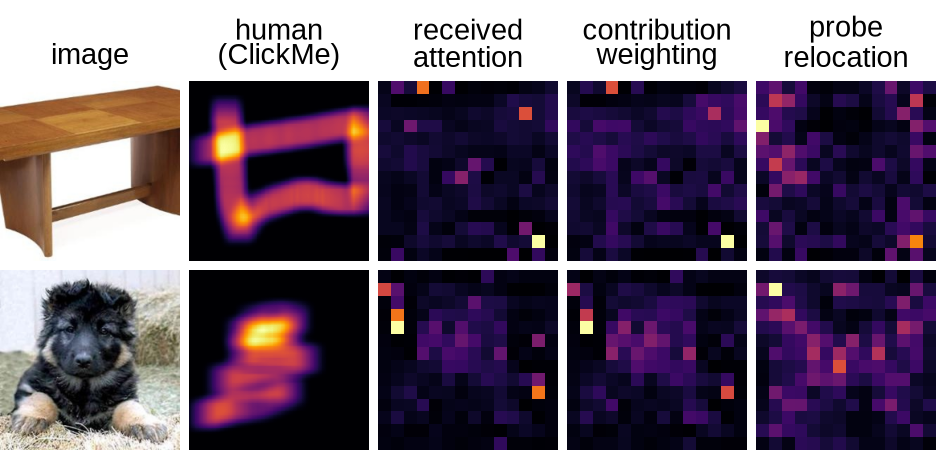
\includegraphics[width=4.7in]{example_maps}
\captionof{figure}{The first two fixed-seed examples, DeiT-S, layers 9--12. Colours show scores min--max normalised within each map; amplitudes are not comparable across panels. These images were not selected for correction gain.}
\label{fig:app-gallery-first}
\end{minipage}\end{center}

\begin{center}\begin{minipage}{\linewidth}
\centering
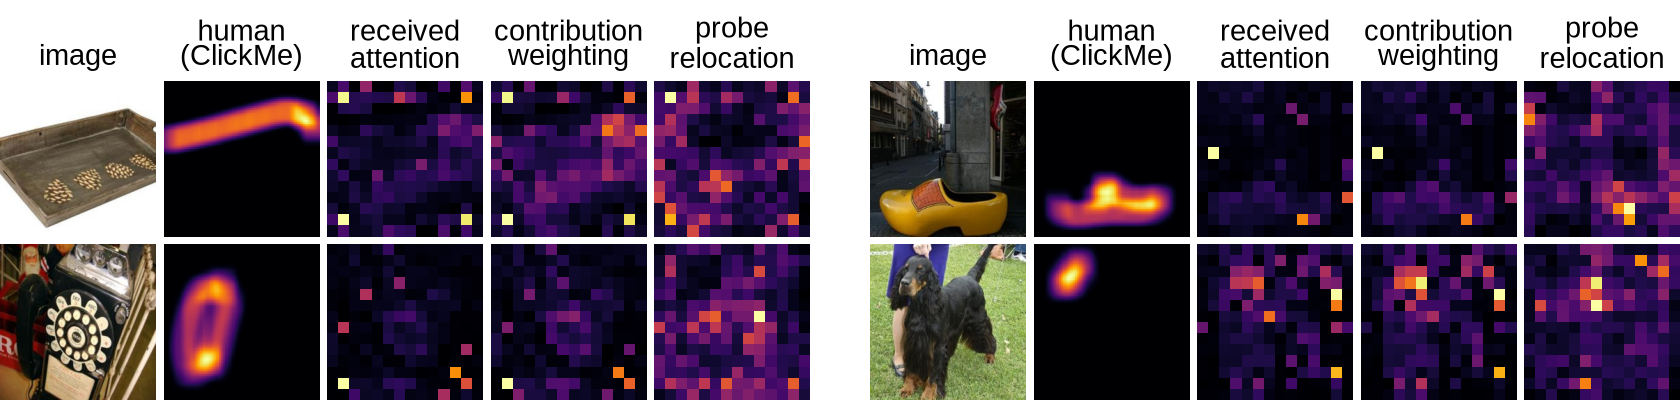
\includegraphics[width=5.5in]{example_maps_more}
\captionof{figure}{DeiT-S on four further ClickMe images, layers 9--12; colours are normalised within each map and do not compare amplitudes across panels.}
\label{fig:app-gallery}
\end{minipage}\end{center}

% =====================================================================================================
\clearpage
\section{Exploratory analyses of norm weighting}\label{app:explore}
\paragraph{Deletion endpoints.} For each image and method, trapezoidal integration uses the original removal budgets, divided by 196. The probability endpoint integrates the probability of the original top-1 class under least-important-first removal minus most-important-first removal. The KL endpoint uses the reverse difference in divergence from the original prediction, so that larger scores again indicate greater separation. For both endpoints the paired curve difference is zero at budget zero. Results are paired over images. These measures have no registered practical margin.
\paragraph{Uncertainty.} Differences are paired by image. Intervals use 1,000 image-bootstrap resamples with seed 0. ClickMe reuses each human map within a batch for its own and another image. Recomputing intervals by sampling the 272 original 64-image batches preserves those dependencies. For C3 relative to zeroing high-norm patches, the resulting ClickMe intervals are [0.021, 0.023] in DeiT-S and [0.016, 0.018] in DeiT-B. All estimates condition on the fixed within-batch pairing and the available checkpoints.
\begin{center}\begin{minipage}{\linewidth}
\captionof{table}{Exploratory endpoint differences (C3 minus comparator). Probability and KL columns give the mean paired area and 95\% image-bootstrap interval over the fixed 2,000-image deletion subset. ClickMe uses the original 17,408 images with batch-bootstrap intervals. KL has units of nats times fraction removed.}
\centering\footnotesize\setlength{\tabcolsep}{3pt}
\begin{tabular}{@{}llrrr@{}}
\toprule
Model & Comparator & Probability area & KL area & ClickMe \\
\midrule
DeiT-S & R0 & 0.014 [0.012, 0.015] & 0.058 [0.050, 0.066] & 0.033 [0.032, 0.034] \\
DeiT-S & Zero high-norm & 0.010 [0.009, 0.012] & 0.041 [0.033, 0.049] & 0.022 [0.021, 0.023] \\
DeiT-B & R0 & 0.022 [0.020, 0.024] & 0.107 [0.096, 0.118] & 0.058 [0.056, 0.059] \\
DeiT-B & Zero high-norm & 0.010 [0.008, 0.012] & 0.048 [0.038, 0.058] & 0.017 [0.016, 0.018] \\
DINO & R0 & 0.000 [$-$0.001, 0.002] & $-$0.003 [$-$0.009, 0.003] & $-$0.001 [$-$0.001, $-$0.001] \\
DINO & Zero high-norm & 0.000 [$-$0.001, 0.002] & $-$0.003 [$-$0.009, 0.003] & $-$0.001 [$-$0.001, $-$0.001] \\
\bottomrule
\end{tabular}

\end{minipage}\end{center}
\begin{center}\begin{minipage}{\linewidth}
\centering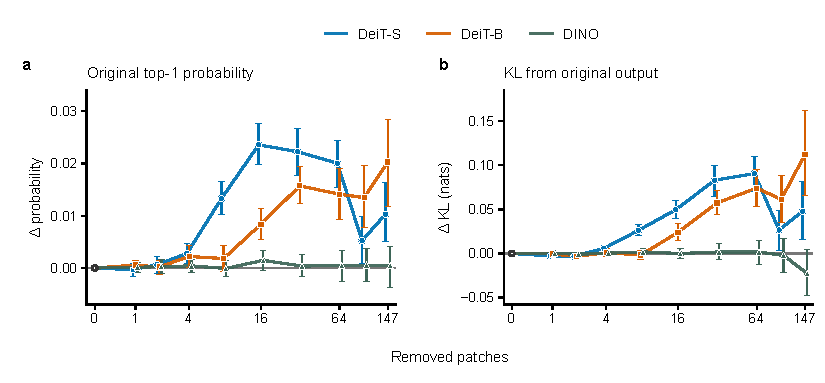
\includegraphics[width=\linewidth]{../../research/v13/endpoints/deletion_curves.pdf}
\captionof{figure}{C3 minus the zero-high-norm control at each original ImageNet-S deletion budget. The probability panel measures least-important-first minus most-important-first target probability. The KL panel reverses the subtraction to express divergence in the same direction. Horizontal positions use a log scale in one plus the number of removed patches, with model-specific offsets for visibility. Intervals are pointwise 95\% paired image-bootstrap intervals over 2,000 images per model. The integrated advantage can coexist with a reversal at a small budget.}
\end{minipage}\end{center}

\clearpage
\subsection{Object geometry and the enrichment scale}
For an image with $M$ valid patches and $k>0$ foreground patches, let ring $r$ contain $m_r$ valid patches of which $f_r$ are foreground. Selecting a patch in this ring contributes $(y-f_r/m_r)/k$ to enrichment, where $y$ is its foreground indicator. Foreground contributions are nonnegative and background contributions are nonpositive. Selecting all $k$ foreground patches therefore attains the maximum
\[
 E_{\max}=1-\frac{1}{k}\sum_{r:m_r>0}\frac{f_r^2}{m_r}\ \le\ 1-\frac{k}{M}.
\]
The inequality follows by Cauchy--Schwarz. It bounds the score itself. The possible change from R0 also depends on R0's starting score. A large raw improvement for small objects can thus reflect properties of both the map and the metric.
\paragraph{Area and centroid displacement.} Object area is the share of valid patch slots labelled foreground. Centroid displacement is the distance from their centroid to the grid centre, in patches. For each checkpoint we computed the empirical quartiles on its finite-geometry images, assigning ties to the lower bin. The DeiT area cut points were 0.158, 0.342 and 0.571. DINO's different crop produced different masks. We paired scores within the same supplementary run and resampled images 2,000 times. In DeiT-S and DeiT-B the largest-minus-smallest area quartile differences in the C3 gain were $-0.090$ and $-0.157$ for enrichment. Comparing the most off-centre with the most central quartile instead gave $+0.057$ and $+0.095$. Area and centroid displacement covary. Among the smallest objects the latter differences were $+0.041$ [0.028, 0.053] and $+0.047$ [0.028, 0.066]. Some joint bins are small and these are observational contrasts.

\paragraph{Metric sensitivity.} After seeing the enrichment gradients we examined patch AUROC under the same quartile cut points. AUROC is the probability that a foreground patch outranks a background patch, counting ties as one half. In the supervised models the gain in AUROC persists across area quartiles (Table~\ref{tab:geometry}). AUROC does not condition on radius, so this comparison changes spatial adjustment as well as how foreground patches are selected. Overall C3-minus-R0 AUROC changes are $+0.028$, $+0.046$ and $-0.005$ for DeiT-S, DeiT-B and DINO.

\paragraph{Historical sample membership.} Archived ImageNet-S files record zero enrichment for all-foreground grids, as the ring formula implies. Counts are 241 such grids for each DeiT and 265 for DINO. An additional 269/275 images, respectively, have zero object area and are excluded from the archived enrichment means. AUROC requires both classes, giving 11,909 DeiT and 11,879 DINO images. Restricting enrichment to that common eligibility changes C3-minus-R0 from 0.03757 to 0.03833 in DeiT-S, 0.06539 to 0.06671 in DeiT-B and $-0.00351$ to $-0.00359$ in DINO. The original verdicts use the archived cohort. In two DeiT-S images the original and supplementary R0 exports differ slightly. The stratified comparisons pair both methods from the supplementary export.

\begin{center}\begin{minipage}{\linewidth}
\captionof{table}{Mean C3 minus R0 by foreground-area quartile on ImageNet-S. Q1 contains the smallest objects. Both metrics use the same within-model cut points. AUROC excludes all-foreground crops.}
\label{tab:geometry}\centering\small\input{geometry_table}
\end{minipage}\end{center}

\clearpage
\subsection{Independent pet-image controls}
The Oxford release provides test filenames and trimaps. We sorted filenames by SHA-256 of the fixed prefix and name (protocol under \texttt{research/v13/spatial/}), taking the first 384. Images were resized on the short side to 248 pixels with bicubic interpolation and centre-cropped to 224. The masks received the same spatial transform with nearest-neighbour interpolation. Label 3 (boundary) was ignored. A patch counted as foreground when at least half its valid pixels were foreground. One crop contained only foreground. Each image and its adjacent partner in hash order exchanged norm rankings. In each within-ring shuffle all heads shared a permutation for that image and layer. The recipient's sorted values, head scales and marginal distributions were preserved by rank transfer. Norm-only sets each head's received attention to its spatial mean before multiplying by its patch-specific length.

All seven readouts were evaluated on identical masks. Primary intervals used 10,000 paired image-bootstrap draws (seed 2026). A follow-up sensitivity check resampled the 192 donor pairs, weighting by the number of eligible images in each draw. C3 minus donor-rank gives 0.0223 [0.0187, 0.0261] in this check. The captured C3 map and logits were checked against the original implementation on the first batch. Each query--patch pair satisfied the triangle bound within numerical tolerance over the run. Public Oxford images and the model weights are available from their original providers. Individual scores, selected IDs, scripts and protocols accompany the source.
\subsection{Last-block CLS value intervention}
A second fixed filename hash selected 128 of the 384 images independently of their scores. At block 12 we cached its input and the unmodified logits. For each patch $j$ we held the original CLS attention weights fixed and removed $t_j=\sum_h a^h_{\mathrm{CLS},j}z_j^h$ from the CLS attention output. The shared projection bias stayed in place. The remaining residual, token-wise MLP, final normalisation and classifier were evaluated for each modified CLS. If $m$ is the margin between the original highest and second-highest logits, the response was $|m_{-j}-m|$ for those same classes. This intervention concerns the contextualised token at that slot. Its input evidence can span multiple image regions.

For each image, we correlated the 196 responses with each unmodified layer-12 readout by Spearman correlation. The means over images were 0.696 (all-query R0), 0.705 (all-query C3), 0.730 (CLS attention), 0.747 (CLS sum of head magnitudes) and 0.756 (CLS net magnitude). The paired CLS-only sum versus all-query C3 difference was 0.041 [0.026, 0.057] with 10,000 image-bootstrap resamples. Explicit interventions in full forward passes on four images and three patch indices each agreed with vectorised logits to within $2.4\times10^{-6}$. The 128-image run took about 3 seconds on the RTX 4060 with inputs cached. The supplied scripts and individual patch responses are under \texttt{research/v13/cls/}.
\input{matched_detail}


\clearpage
\section{Key parts of the code}
\label{app:code}

Given the attention $a_{ij}^h$ and values $v_j^h$ of a layer, the readings are:

\begin{lstlisting}[language=Python]
def received_and_contribution(p, v, w_o, prefix=1):
    # p: [B,H,T,T]; v: [B,H,T,d]; w_o: [D,H,d]
    # T includes CLS; values include the value-projection bias.
    gram = torch.einsum('dhe,dhf->hef', w_o, w_o)
    length = torch.einsum('bhne,hef,bhnf->bhn', v, gram, v)
    length = length.clamp_min(0).sqrt()
    received = p.sum(2)  # sum over queries
    s = received.sum(1)[:, prefix:]
    c = (received * length).sum(1)[:, prefix:]
    return s, c

def relocate(s, probs):  # source j to predicted position p
    return torch.einsum('bj,bjp->bp', s, probs)
\end{lstlisting}

For the independent pet experiment, the following operations compare two weights for the same source patch. Here $a$ has axes (image, head, query, patch), and $z$ contains each head's projected value vector. The implementation processes queries in chunks.
\begin{lstlisting}[language=Python]
# Own lengths versus the same lengths in a donor image's spatial order
length = z.norm(dim=-1)                         # [B, H, 196]
order = donor_length.argsort(dim=-1)
borrowed = torch.empty_like(length).scatter(-1, order, length.sort(-1).values)
received = a.sum(dim=2)
own_map = (received * length).sum(dim=1)
donor_map = (received * borrowed).sum(dim=1)

# Magnitude after summing the head vectors for each query and patch
net_map = sum(torch.einsum('bhij,bhjd->bijd', chunk, z).norm(dim=-1).sum(1)
              for chunk in a.split(32, dim=2))
\end{lstlisting}

For the final-block intervention we hold the attention matrix fixed. This excerpt from the full-forward check removes one patch's term from the CLS query. The output projection retains its bias and the rest of the model runs normally.
\begin{lstlisting}[language=Python]
# p: [batch, head, query, source]; v: [batch, head, source, head_dim]
head_out = p @ v
head_out[:, :, 0, :] -= p[:, :, 0, source_patch + 1, None] * v[:, :, source_patch + 1, :]
full = head_out.transpose(1, 2).reshape(batch, tokens, -1)
return attn.proj_drop(attn.proj(attn.norm(full)))
\end{lstlisting}

\end{document}
